% !TEX root = BioInspired.tex

\chapter{Cellular Automata - Text Chapter 8}

\section{Problem 8.3}

Implement one of the Problems on the StarLogo website -- we chose to do the rabbit and grass simulation.

\subsection{Problem Information}

The rabbit and grass simulation proposes a plane with randomly scattered grass and rabbits.  Over time, the patches without grass grow grass and the rabbits move around, eating the grass off of the grassy patches.  As the rabbits consume the grass, they gain energy.  Once they reach a sufficient energy level, they bud off a second rabbit, which goes off on its own and eatis and reproduces by itself.

The Rabbits all move randomly and lose a slight amount of energy with every movement.  If they run out of energy, they die.

There are a handful of parameters which can be passed into the simulation.  The hatch threshold is the amount of energy required for reproduction in a single rabbit.  The starvation rate is the amount of energy that bunnies lose at every movement.  The grass growth rate is the chance that grass will grow in any given square in any given time step.  The maximum iterations is the maximum number of steps that the simulation will run.

\subsection{Algorithm Description}

We created a Bunny class, which held the position and energy of the bunnies.  In the time step, the grass matrix was updated by growing grass in each tile with a certain probability.  However, before the grass was grown, the bunnies were iterated through.  Their various bodily functions and movements were processed and their energy was modified, and then at the end of each bunny's iteration, it would be marked as dead if its energy

was below zero.  At the end of the time step, all bunnies which were marked as dead were removed.  At the end of each step, the pyplot was updated with the grass and grassless spots, drawing red spots where there were bunnies.

\subsection{Results}

This was simple and fun, and different settings yielded very different results.  Setting the starvation rate to something very low - like .05 - and setting the growth rate to something also very low - like .001 - give a good example of a fluctuating population.  The default parameters give a fairly generic example.  If the growth rate was too high in relation to the starvation rate, then the bunnies would exponentially overpopulate.  If the converse was
 true, then the rabbits would go extinct.  Decreasing the hatch threshold speeds up the whole simulation.
  

\begin{figure}[tbh]
\begin{center}
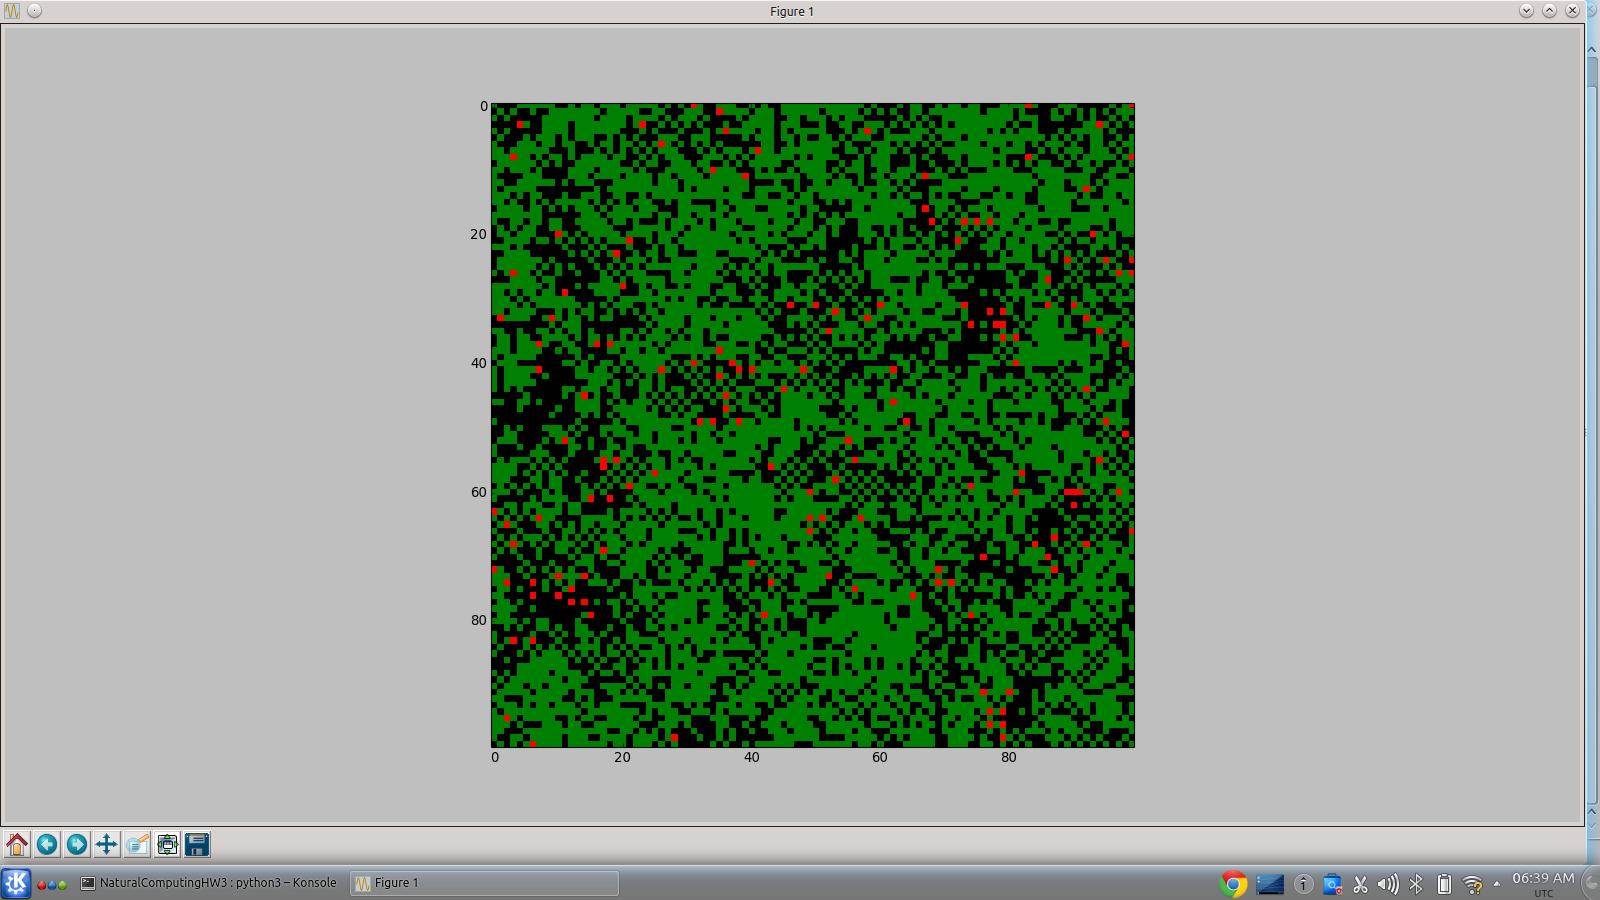
\includegraphics[width=0.75\textwidth]{rabbits1.png}
\end{center}
\caption{The Rabbit Simulation\label{fig:gprun}}
\end{figure}



\section{Problem 8.4}

Implement Conway's Game of Life

\subsection{Problem Information}

Conway's Game of Life is a well-known cellular automata simulation of which Derek was already familiar.  This made testing and verification easy, although the main challenge was in implementing a fast solution.  

Conway's Game of Life is a simulation with four simple rules.  Firstly, any cell with more than three live neighbors dies of overcrowding.  Secondly, any cell with exactly three neighbors comes to life.  Thirdly, any cell with less than two neighbors dies of starvation.  Lastly, any live cell with two or three neighbors lives on to the next generation.

\subsection{Algorithm Description}

We implemented a grid which was drawn by pyplot, setting live cells to black and dead cells to white.  Following each of those rules iteratively, we updated the cell grid each generation.  

The number of neighbors for each cell was calculated by convolving the grid with a 3x3 mask.

\subsection{Results}

The result was an adjustable game of life accurate to the specifications.   The first argument should be start.txt, the second should be the generations/second - 10 is usually good.  The third argument should be the maximum number of generations, which is entirely up to the user.  Entering a very high number is advised. The starting configuration file is structured so the first line has the height and width of the playing field Subsequent lines are rows in the playing field.  0s are cells which are dead, and 1s are cells which are alive.

\begin{figure}[tbh]
\begin{center}
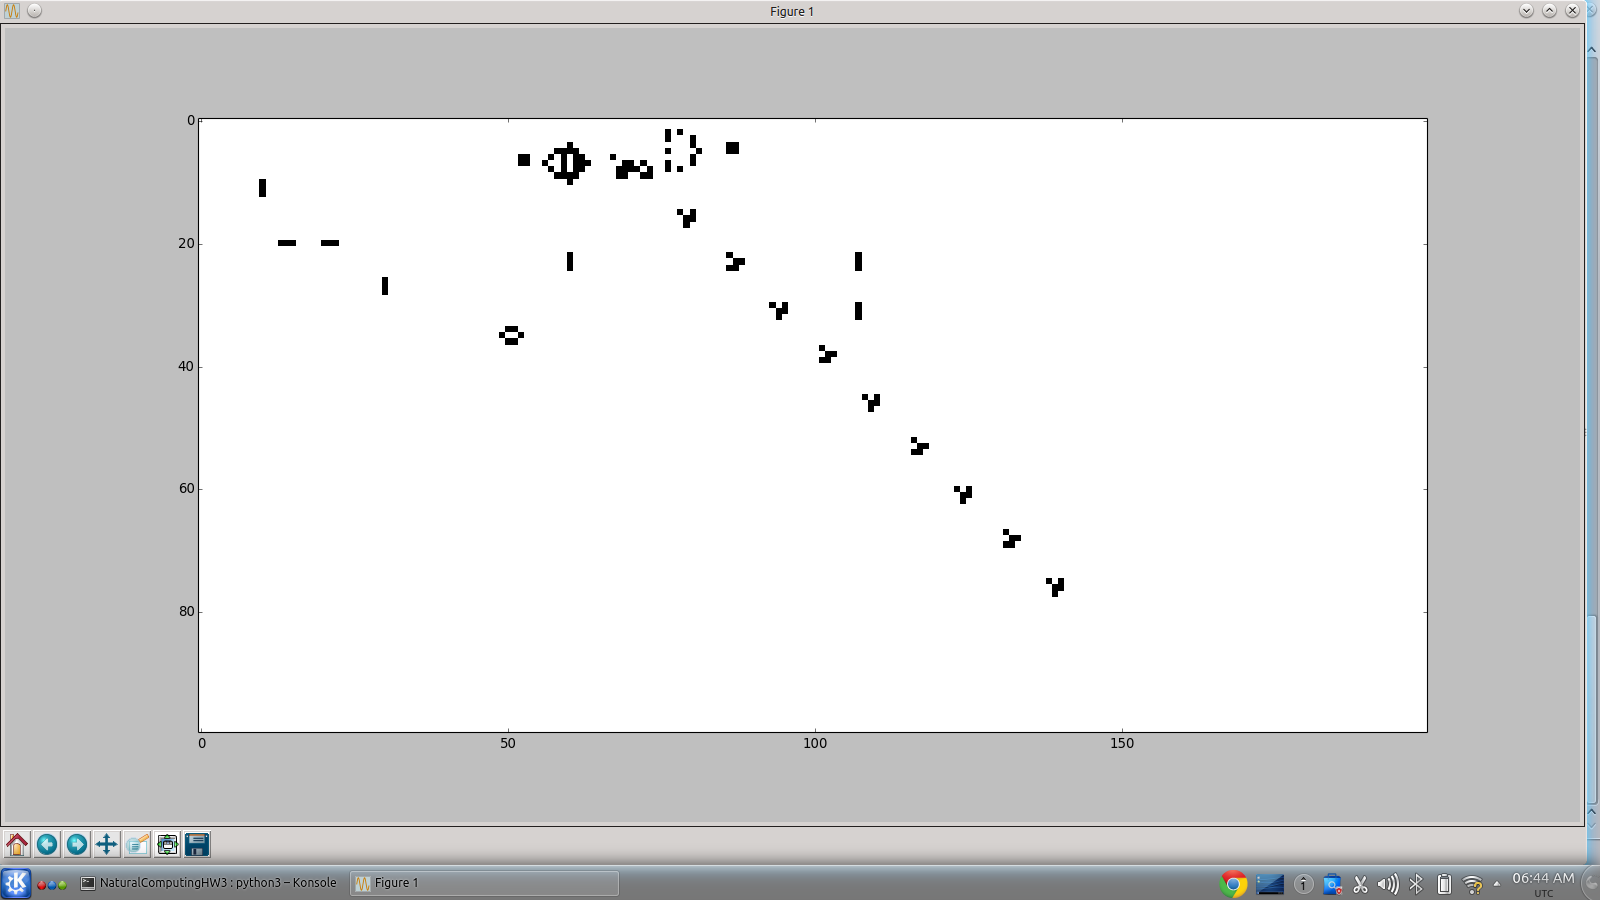
\includegraphics[width=0.75\textwidth]{glidergun.png}
\end{center}
\caption{A Glider Gun in Conway's Game of Life\label{fig:gprun}}
\end{figure}
